\documentclass[a4paper]{scrartcl}
\usepackage[greek,ngerman]{babel}
\usepackage{fontspec,xltxtra,xunicode}
\usepackage{graphicx}
\usepackage{amsmath}
\usepackage{amssymb}
\usepackage{wasysym}
\usepackage{wrapfig}
\usepackage{caption}
\usepackage{lmodern}
\usepackage{csquotes}
\usepackage{subcaption}
\usepackage[pdfborder={0 0 0}]{hyperref}
\usepackage{cleveref}[2012/02/15]
\usepackage[backend=biber]{biblatex}
\addbibresource{report.bib}
\defaultfontfeatures{Ligatures=TeX}
\setmainfont[
  Path=baskervald/OTF/,
  BoldFont=*-Bold,
  ItalicFont=*-Italic,
  BoldItalicFont=*-BoldItalic,
  SmallCapsFont=BaskervaldSmallCaps.ttf
]{BaskervaldADFStd}

\newfontfamily\oghamfont[
  Path=BabelStoneOghamFonts/,
  Extension=.ttf,
  ItalicFont=BabelStoneOghamI
]{BabelStoneOghamR}

\newfontfamily\ipafont[Path=LinuxLibertine/]{LinBiolinum_Rah.ttf}
\newfontfamily\runicfont[Path=titus-runic/]{TITUSCBZ.TTF}

\makeatletter
\hypersetup{
  pdftitle={\@title},
  pdfauthor={\@author},
  pdfsubject={Runen, Ogham-Schrift und das Gotische Alphabet},
  pdfcreator={\LaTeX},
  pdfkeywords={Germanisch, Schriftsystem, Runen, Alphabet, Runische Zeichnungen, Ogham-Schrift, Gotisches Alphabet},
  pdfview=FitV,
  pdflang={de-AT},
  unicode,
  breaklinks
}
\makeatother

\crefformat{footnote}{#2\footnotemark[#1]#3}

\newcommand{\character}[1]{\textsc{#1}}
\captionsetup{justification=centering}


\author{Lukas Prokop, *}
\title{Runen und die Ogham-Schrift}
\date{Jänner 2015}

\begin{document}
\maketitle
\tableofcontents

\section{Grundlagen}

\emph{Erster Teil der Gruppenarbeit fehlt bisher.}

\begin{table}[p]
  \small
  \begin{center}
    \begin{tabular}{clclcl}
      {\runicfont ᚠ} & \textsc{Fehu Feoh Fe F} &
      {\runicfont ᚡ} & \textsc{V} &
      {\runicfont ᚢ} & \textsc{Uruz Ur U} \\
      {\runicfont ᚣ} & \textsc{Yr} &
      {\runicfont ᚤ} & \textsc{Y} &
      {\runicfont ᚥ} & \textsc{W} \\
      {\runicfont ᚦ} & \textsc{Thurisaz Thurs Thorn} &
      {\runicfont ᚧ} & \textsc{Eth} &
      {\runicfont ᚨ} & \textsc{Ansuz A} \\
      {\runicfont ᚩ} & \textsc{Os O} &
      {\runicfont ᚪ} & \textsc{Ac A} &
      {\runicfont ᚫ} & \textsc{Aesc} \\
      {\runicfont ᚬ} & \textsc{Long-Branch-Oss O} &
      {\runicfont ᚭ} & \textsc{Short-Twig-Oss O} &
      {\runicfont ᚮ} & \textsc{O} \\
      {\runicfont ᚯ} & \textsc{Oe} &
      {\runicfont ᚰ} & \textsc{On} &
      {\runicfont ᚱ} & \textsc{Raido Rad Reid R} \\
      {\runicfont ᚲ} & \textsc{Kauna} &
      {\runicfont ᚳ} & \textsc{Cen} &
      {\runicfont ᚴ} & \textsc{Kaun K} \\
      {\runicfont ᚵ} & \textsc{G} &
      {\runicfont ᚶ} & \textsc{Eng} &
      {\runicfont ᚷ} & \textsc{Gebo Gyfu G} \\
      {\runicfont ᚸ} & \textsc{Gar} &
      {\runicfont ᚹ} & \textsc{Wunjo Wynn W} &
      {\runicfont ᚺ} & \textsc{Haglaz H} \\
      {\runicfont ᚻ} & \textsc{Haegl H} &
      {\runicfont ᚼ} & \textsc{Long-Branch-Hagall H} &
      {\runicfont ᚽ} & \textsc{Short-Twig-Hagall H} \\
      {\runicfont ᚾ} & \textsc{Naudiz Nyd Naud N} &
      {\runicfont ᚿ} & \textsc{Short-Twig-Naud N} &
      {\runicfont ᛀ} & \textsc{Dotted-N} \\
      {\runicfont ᛁ} & \textsc{Isaz Is Iss I} &
      {\runicfont ᛂ} & \textsc{E} &
      {\runicfont ᛃ} & \textsc{Jeran J} \\
      {\runicfont ᛄ} & \textsc{Ger} &
      {\runicfont ᛅ} & \textsc{Long-Branch-Ar Ae} &
      {\runicfont ᛆ} & \textsc{Short-Twig-Ar A} \\
      {\runicfont ᛇ} & \textsc{Iwaz Eoh} &
      {\runicfont ᛈ} & \textsc{Pertho Peorth P} &
      {\runicfont ᛉ} & \textsc{Algiz Eolhx} \\
      {\runicfont ᛊ} & \textsc{Sowilo S} &
      {\runicfont ᛋ} & \textsc{Sigel Long-Branch-Sol S} &
      {\runicfont ᛌ} & \textsc{Short-Twig-Sol S} \\
      {\runicfont ᛍ} & \textsc{C} &
      {\runicfont ᛎ} & \textsc{Z} &
      {\runicfont ᛏ} & \textsc{Tiwaz Tir Tyr T} \\
      {\runicfont ᛐ} & \textsc{Short-Twig-Tyr T} &
      {\runicfont ᛑ} & \textsc{D} &
      {\runicfont ᛒ} & \textsc{Berkanan Beorc Bjarkan B} \\
      {\runicfont ᛓ} & \textsc{Short-Twig-Bjarkan B} &
      {\runicfont ᛔ} & \textsc{Dotted-P} &
      {\runicfont ᛕ} & \textsc{Open-P} \\
      {\runicfont ᛖ} & \textsc{Ehwaz Eh E} &
      {\runicfont ᛗ} & \textsc{Mannaz Man M} &
      {\runicfont ᛘ} & \textsc{Long-Branch-Madr M} \\
      {\runicfont ᛙ} & \textsc{Short-Twig-Madr M} &
      {\runicfont ᛚ} & \textsc{Laukaz Lagu Logr L} &
      {\runicfont ᛛ} & \textsc{Dotted-L} \\
      {\runicfont ᛜ} & \textsc{Ingwaz} &
      {\runicfont ᛝ} & \textsc{Ing} &
      {\runicfont ᛞ} & \textsc{Dagaz Daeg D} \\
      {\runicfont ᛟ} & \textsc{Othalan Ethel O} &
      {\runicfont ᛠ} & \textsc{Ear} &
      {\runicfont ᛡ} & \textsc{Ior} \\
      {\runicfont ᛢ} & \textsc{Cweorth} &
      {\runicfont ᛣ} & \textsc{Calc} &
      {\runicfont ᛤ} & \textsc{Cealc} \\
      {\runicfont ᛥ} & \textsc{Stan} &
      {\runicfont ᛦ} & \textsc{Long-Branch-Yr} &
      {\runicfont ᛧ} & \textsc{Short-Twig-Yr} \\
      {\runicfont ᛨ} & \textsc{Icelandic-Yr} &
      {\runicfont ᛩ} & \textsc{Q} &
      {\runicfont ᛪ} & \textsc{X} \\
      {\runicfont ᛫} & \textsc{Single Punctuation} &
      {\runicfont ᛬} & \textsc{Multiple Punctuation} &
      {\runicfont ᛭} & \textsc{Cross Punctuation} \\
      {\runicfont ᛮ} & \textsc{Arlaug Symbol} &
      {\runicfont ᛯ} & \textsc{Tvimadur Symbol} &
      {\runicfont ᛰ} & \textsc{Belgthor Symbol}
    \end{tabular}
    \caption{Runen als Grapheme und deren Bezeichnung nach Unicode}
  \end{center}
\end{table}

% * Grundlagen
%  - zeitliche, historische und geografische Einordnung
%  - Skizzierung der Völkerniederlassungen im damaligen Europa?
\subsection{Geschichte}
\subsection{Älteste Funde}
\section{Philologie}
\subsection{Die Schrift}
% * Philologie
%  - Runenschrift als Begriff- und Runenschrift, Schriftrichtung
%  - Überblick über das Alphabet
%  - Ähnlichkeiten zu anderen Schriften?
%  - Germanische Sprachen, Eigenschaften, Geschichte, Verbreitung

\newpage

\section{Anwendung}
\emph{Geschrieben von Lukas Prokop.}

\subsection{Die Sage von Odin und der Entstehung der Runen}
%
Odin war die Hauptfigur aller Götter in der nordischen Mythologie (nach Wagner neudeutsch \glqq Wotan\grqq). Die Germanen glaubten, dass Odin die Runen entworfen und den Menschen geschenkt hat. Die Edda-Lieder sind in altisländischer Sprache überliefert und 164 enthaltene eddische Lieder (bezeichnet als \enquote{Hávamál}) erzählen von vorchristlichen germanischen Göttern und Helden. Die Hávamál erzählt in den Worten Odins von der Entstehung der Runen~\cite{havamal}:

\begin{table}[!ht]
  \begin{center}
    \begin{tabular}{lp{30pt}l}
      Veit ek, at ek hekk   && Ich weiß, dass ich hing \\
      vindga meiði á        && An windigem Baum \\
      nætr allar níu,       && neun ganze Nächte, \\
      geiri undaðr          && vom Speer verwundet \\
      ok gefinn Óðni,       && und Odin geweiht, \\
      sjalfr sjalfum mér,   && ich selbst mir selbst, \\
      á þeim meiði,         && an diesem Baum, \\
      er manngi veit        && von dem niemand weiß \\
      hvers af rótum renn.  && aus welcher Wurzel er sprießt.
    \end{tabular}
    \caption{Vers~138 der Hávamál (Beginn Odins Runenlied)}
  \end{center}
\end{table}
%
\begin{table}[!ht]
  \begin{center}
    \begin{tabular}{lp{30pt}l}
      Við hleifi mik sældu  && Ich gab mich hin nicht für Brot \\
      né við hornigi;       && und nicht für Hornvieh, \\
      nýsta ek niðr,        && ich spähte nach unten, \\
      nam ek upp rúnar,     && nahm Runen auf, \\
      æpandi nam,           && laut lernte ich sie, \\
      fell ek aftr þaðan.   && fiel wieder von dort.
    \end{tabular}
    \caption{Vers~139 der Hávamál (mit Erwähnung der Runen [rúnar])}
  \end{center}
\end{table}

Hierbei ist zu beachten, dass mit Runen nicht die Menge an Zeichen gemeint ist, sondern diese Bezeichnung stets auf magisch-mythische Sprüche bezogen zu verstehen ist. So wird die 4. Zeile etwa auch als \enquote{I lifted the secrets}\footnote{\enquote{secrets} ist zu deutsch als Geheimnis zu übersetzen. Es sei darauf hingewiesen, dass bereits \enquote{rûna} im Altsächsischen Geheimnis bedeutet~\cite[S. 1]{düwel}.} übersetzt~\cite{havamal-vers-139}.

\subsection{Die Runen in der germanischen Kultur}
%
Runen wurden in verschiedenen Kontexten verwendet.

\begin{figure}[!ht]
  \begin{minipage}{0.5\textwidth}
    \begin{itemize}
      \item Besitzangabe
      \item Herstellerinschriften
      \item Rechnungen
      \item Magische Anreden an Geister und Dämonen
    \end{itemize}
  \end{minipage}
  \begin{minipage}{0.5\textwidth}
    \begin{itemize}
      \item Kultische / rituelle Formeln
      \item Sakrale Kommunikation mit/von Göttern
      \item Totengedenken
      \item Private Nachrichten
    \end{itemize}
  \end{minipage}
\end{figure}

Seit der Entstehung der Schrift wurde sie im Bereich der Verwaltung eingesetzt, um Besitztum und Rechte zu dokumentieren. Selbiges gilt für den Handel, um Warenflüsse aufzuzeichnen und Schuldscheine auszustellen. Beim Totengedenken kommt etwas Besonderes hinzu: Die reisefreudigen Wikinger zogen oft in den Krieg in der Ferne und beim Ableben wurden Totensteine erstellt und beschrieben, um Kriegern ihre letzte Ehre zu erweisen. Private Nachrichten und sakrale Notizen finden sich bevorzugt auf tragbaren Medien, die auch eine geringere Lebensdauer besitzen.

Düwel betont die Reichweite der Runenverwendung. Die gefundenen Texte umfassen Texte aller Facetten, \enquote{die von der inbrünstigen Bitte bis zur groben Obszönität reichen}~\cite{düwel}.

\subsection{Zusammenhang mit dem Mythischen}
%
Die Germanen besaßen einen starken Gottheitskult. Nach ihrer Auffassung kamen die Götter aus 9 verschiedenen Welten und waren verschiedenen Typus: Naturgeister, Ungeheuer, Zwerge und Dämonen.

Signifikant ist in diesem Zusammenhang die Verwendung der Metapher \enquote{alu} ({\runicfont ᚨᛚᚢ}). Runentexte konnte aufgrund ihres Inhalts ihr Kontext zugewiesen werden. So kommt in privaten Nachrichten bzw. Liebesbriefen häufig das Adjektiv \enquote{Liebste} bzw. \enquote{Liebster} vor. Mythische Formeln können anhand der alu-Metapher erkannt werden. Dieses Schlüsselwort wird an beliebiger Stelle (bevorzugt jedoch am Ende\footnote{Es lässt sie vermutlich mit dem christlichen Amen im Gebet vergleichen. Nach Düwel~\cite[S. 36]{düwel} wurde es in der frühen Forschung als \enquote{Abwehr von Grabjägern oder Wiedergängern} interpretiert, wenn es an sakralen Elementen angebracht wurde. In der neueren Forschung geht man davon aus, dass es nicht nur zur Abschreckung sondern auch als \enquote{Kennzeichnung einer Kultstätte} verwendet wurde. \enquote{alu} bezeichnete ursprünglich einen Ekstasezustand~\cite[S. 36]{düwel}.}) platziert. Die Verwendung dieser Metapher kann beispielhaft am Lindholm Amulett (siehe Abbildung~\ref{fig:lindholm}) angesehen werden.
%
\begin{figure}[p]
  \begin{center}
    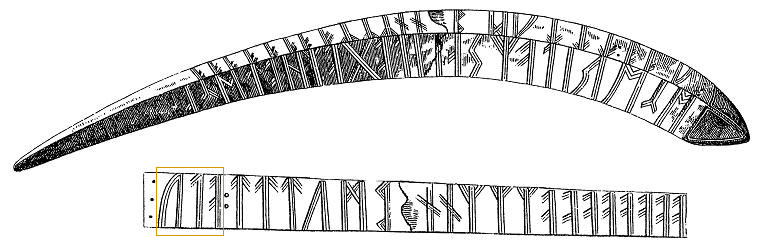
\includegraphics[width=\textwidth]{images/lindholm_amulet.jpg}
    \caption{Lindholm Amulett~\cite{lindholm} (Stephens, 1884) \\ die Hervorhebung markiert die {\glqq alu\grqq} Metapher}
    \label{fig:lindholm}
  \end{center}
\end{figure}

\subsection{Geheimrunen}
%
Eine frühe Form der Verschlüsselung kann an den Geheimrunen erkannt werden. Düwel~\cite[S. 182]{düwel} identifiziert mehrere Verschlüsselungsarten (siehe Tabelle~\ref{tab:encodings}).

\begin{table}[!t]
  \begin{minipage}{0.5\textwidth}
    \begin{itemize}
      \item Umstellung
      \item Abkürzung
      \item Auslassung von inlautenden Vokalen
      \item Namensangabe in einem Runenkreuz
    \end{itemize}
  \end{minipage}
  \begin{minipage}{0.5\textwidth}
    \begin{itemize}
      \item Teilhafte Rückwärtsschreibung
      \item Hinzufügen runenähnlicher Zeichen als Vokale
      \item Verschieberunen
    \end{itemize}
  \end{minipage}
  \caption{Auflistung einiger Verschlüsselungsarten nach Düwel~\cite[S. 182]{düwel}}
  \label{tab:encodings}
\end{table}

Im Folgenden soll folgendes kreative Verfahren illustriert werden: Die Runen werden in 3 Gruppen eingeteilt (siehe Tabelle~\ref{tab:encode}).

\begin{table}[!t]
  \begin{center}
    \begin{tabular}{clll}
      Klasse 1: & f, u, {\runicfont ᚦ}, {\runicfont ą}, r, k \\
      Klasse 2: & h, n, i, a, s \\
      Klasse 3: & t, b, m, l, \textsc{r}
    \end{tabular}
    \caption{Einteilung der Runen in 3 Klassen zur Verschlüsselung~\cite[S. 183]{düwel}}
    \label{tab:encode}
  \end{center}
\end{table}

Nun handelt es sich beim Buchstaben \enquote{f} um das erste Zeichen der ersten Klasse; notiert als \enquote{1 / 1}. Diese Notation wurde jetzt wiederum durch Symbole kodiert. Man nutzt hierzu Strichmännchen in verschiedenen Positionen oder die Ausrichtung von Bartsträhnen in der graphischen Darstellung des kodierten Symbols.

\section{Ogham-Schrift}
\subsection{Zeitliche und geografische Einordnung}
%
Die Ursprünge der Ogham-Schrift reichen in das 1. Jahrhundert nach Christus zurück~\cite{ogham-heidnisch1}.
Die meisten heutigen Zeugnisse der Ogham-Schrift stammen allerdings aus der Zeit zwischen dem 4. und 5.~Jhdt. n.~Chr.
Es handelt sich fast ausschließlich um Steininschriften, die Namensnennungen aufweisen. Diese Steine wurden etwa als Grabsteine oder zur Besitzangabe verwendet.

\begin{figure}[t]
  \begin{center}
    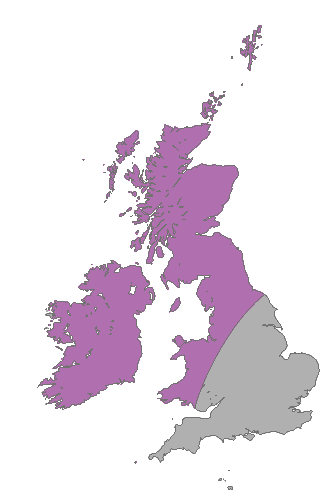
\includegraphics{images/ogham_areas.pdf}
    \caption{Violette Bereiche geben Bereiche mit Verbreitung der Ogham-Schrift an}
  \end{center}
\end{figure}

Die Ogham-Schrift [{\footnotesize IPA:} {\ipafont ˈɔɣam}] wurde im keltischen Kulturbereich verwendet und Relikte finden sich in den heutigen Gebieten Irlands, Schottlands und dem westlichen England. Die Oghamschrift war eine wichtige Grundlage zur Erforschung der archaisch-irischen Sprache bzw. ihrem Nachfolger Altirisch.

Bezüglich des Ursprungs des Namens Ogham für die Schrift gibt es verschiedene Theorien. So lautet eine Theorie etwa, dass der altirische Gott der Redekunst namens \foreignlanguage{greek}{\ipafont Ὄγμιος} sich für die Namensgebung verantwortlich zeichnet. 

Fraglich bleibt außerdem ob die Ogham-Schrift der heidnischen Religionsauffassung zuzuordnen ist~\cite{ogham-heidnisch1,ogham-heidnisch2}. Obwohl Namensnennungen mit dem Titel Priester gefunden wurden~\cite[S. 36]{düwel}, ist die Religionspraxis der Kelten weitgehend unklar. Vermutlich dürfte es sich um eine schwach ausgeprägte Mischung verschiedener Religionen handeln. So wurden einige Götter der römischen Theologie entlehnt~\cite{ogham-religion} (vergleiche Teutates / Mercurius, Cernunnos / Jupiter, Grannus / Apollo und Lenus / Mars). Ursache für die Unklarheiten ergeben sich vor allem daraus, dass die religiöse Lehre der Kelten durch mündliche Übertragung und nicht schriftlich erfolgt ist.

Das TITUS-Projekt~\cite{ogham-titus} (\glqq Thesaurus Indogermanischer Text- und Sprachmaterialien\grqq, 1996--2001) beinhaltet eine große Sammlung von Dokumenten indogermanischer Kultur. 79~Ogham-Inschriften sind archiviert, klassifiziert und entziffert vorzufinden.

\begin{table}[p]
  \begin{center}
    \begin{subfigure}[c]{0.24\textwidth}
      \centering
      \begin{tabular}{cl}
        {\oghamfont ᚁ} & \textsc{Beith} \\
        {\oghamfont ᚂ} & \textsc{Luis} \\
        {\oghamfont ᚃ} & \textsc{Fearn} \\
        {\oghamfont ᚄ} & \textsc{Sail} \\
        {\oghamfont ᚅ} & \textsc{Nion} \\
      \end{tabular}
      \caption{Aicme Beithe}
    \end{subfigure}
    \begin{subfigure}[c]{0.24\textwidth}
      \centering
      \begin{tabular}{cl}
        {\oghamfont ᚆ} & \textsc{Uath} \\
        {\oghamfont ᚇ} & \textsc{Dair} \\
        {\oghamfont ᚈ} & \textsc{Tinne} \\
        {\oghamfont ᚉ} & \textsc{Coll} \\
        {\oghamfont ᚊ} & \textsc{Ceirt} \\
      \end{tabular}
      \caption{Aicme hÚatha}
    \end{subfigure}
    \begin{subfigure}[c]{0.24\textwidth}
      \centering
      \begin{tabular}{cl}
        {\oghamfont ᚋ} & \textsc{Muin} \\
        {\oghamfont ᚌ} & \textsc{Gort} \\
        {\oghamfont ᚍ} & \textsc{nGéadal} \\
        {\oghamfont ᚎ} & \textsc{Straif} \\
        {\oghamfont ᚏ} & \textsc{Ruis} \\
      \end{tabular}
      \caption{Aicme Muine}
    \end{subfigure}\vspace{30pt}
    \begin{subfigure}[c]{0.24\textwidth}
      \centering
      \begin{tabular}{cl}
        {\oghamfont ᚐ} & \textsc{Ailum} \\
        {\oghamfont ᚑ} & \textsc{Onn} \\
        {\oghamfont ᚒ} & \textsc{Úr} \\
        {\oghamfont ᚓ} & \textsc{Eadhadh} \\
        {\oghamfont ᚔ} & \textsc{Iodhadh} \\
      \end{tabular}
      \caption{Aicme Ailme}
    \end{subfigure}
    \begin{subfigure}[c]{0.3\textwidth}
      \centering
      \begin{tabular}{cl}
        {\oghamfont ᚕ} & \textsc{Éabhadh} \\
        {\oghamfont ᚖ} & \textsc{Ór} \\
        {\oghamfont ᚗ} & \textsc{Uilleann} \\
      \end{tabular}
      \caption{Forfeda Teil 1}
    \end{subfigure}
    \begin{subfigure}[c]{0.3\textwidth}
      \centering
      \begin{tabular}{cl}
        {\oghamfont ᚘ} & \textsc{Ifín} \\
        {\oghamfont ᚙ} & \textsc{Eamhancholl} \\
        {\oghamfont ᚚ} & \textsc{Peith} \\
      \end{tabular}
      \caption{Forfeda Teil 2}
    \end{subfigure}
    \begin{subfigure}[c]{0.3\textwidth}
      \centering
      \begin{tabular}{cl}
        {\oghamfont ᚛} & \textsc{Eite} \\
        {\oghamfont ᚜} & \textsc{Eite Thuathail} \\
        {\oghamfont  } & \textsc{Spás} \\
      \end{tabular}
      \caption{Satzzeichen}
    \end{subfigure}
    \caption{Die Schriftzeichen der Ogham-Schrift}
    \label{fig:ogham-chars}
  \end{center}
\end{table}

\subsection{Die 29 Zeichen der Oghamschrift}
%
In Abbildung~\ref{fig:ogham-chars} sind alle Zeichen der Oghamschrift aufgelistet. Die Zeichen wurden entlang der Kante der Steine notiert und die Schreibrichtung verlief dabei von unten nach oben. Falls der Platz nicht ausreichte, wurde in Spalten von links nach rechts fortgesetzt. Alle Zeichen basieren auf Namen von Baumarten und man kann eine Klassifikation vornehmen. Die ersten 20 Zeichen besitzen eine auffällige Struktur: In einem System von $4\times 5$ Zeichen wird mit Hilfe von Stäbchen von 1 bis 20 gezählt. Dieses System (bzw. deren Basis 20) ist auf die Zählung von Waren und Gütern im Handel zurückzuführen. Folglich wird Ogham nicht als eigenständiges Alphabet betrachtet. Es handelt sich um eine andere Kodierungsform\footnote{Eine Kodierungsform, welche ihre Zeichen einer Zählweise entlehnt.} einer gebräulichen Sprache der damaligen Zeit wie Griechisch oder Latein. 

Illustriert werden kann dies anhand von Kerbholzfunden~\ref{fig:tally-stick}. Dabei werden Kerben in einem Kerbholz verwendet, um zu zählen. Der gespreizte Abstand zwischen dem Zeigefinger und dem Daumen dient dabei als Arbeitsbreite. Kerben im Abstand der Breite einer Handfläche repräsentieren 1000~Pfund. Eine Daumenbreite wird für 100~Pfund verwendet und die Breite des kleinen Fingers für 20~Pfund. Ein aufgequollenes Gerstenkorn notiert eine einzelne Geldeinheit. Man beachte die Definition von 20~Pfund und die fehlende Definition für 10~Pfund; das heutig übliche Zählsystem im germanischen Sprachraum basierend auf den 10~Fingern einer Hand. Um die Schuld oder den Warenaustausch nachweisbar zu halten, wird das Kerbholz in zwei Teile gebrochen und das \glqq Dokument\grqq{} an beide Parteien verteilt.

\begin{figure}[t]
  \begin{center}
    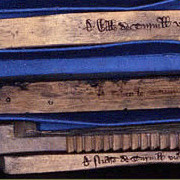
\includegraphics[width=120pt,height=120pt]{images/tally_stick.jpg}
    \caption{Spaltkerbholzfund aus dem 13. Jahrhundert~\cite{tally-sticks}}
    \label{fig:tally-stick}
  \end{center}
\end{figure}

Die Schrift teilt sich 5 Klassen auf (vgl. Tabelle~\ref{fig:ogham-chars}). \emph{Aicme Beithe}, \emph{Aicme hÚatha}, \emph{Aicme Muine}, \emph{Aicme Ailme}, \emph{Forfeda} und \emph{Satzzeichen}. Die ersten 4 Klassen sind durch ihre Zählzeichen von eins bis fünf charakterisiert. Jeder Buchstabe ist mit dem ersten Laut seines Namens auszusprechen. Die Aussprache von \character{Uath} und \character{Straif} sind jedoch unbekannt. Die Forfeda ist eine Menge von 5 Zeichen, welche im Mittelalter hinzugefügt wurden.

\glqq Auraicept Na N'{\'E}ces, the Scholars' Primer\grqq{}~\cite{auraicept1917} wird als Grundlagenarbeit zur Interpretation der Forfeda-Symbole betrachtet. Colin Murray und Liz haben weitere Forschungsarbeit betrieben und interpretieren diese Symbole der Reihe nach auch als Ch\footnote{\label{foot:alt}als Alternative}, Oi/Th, Pe\cref{{foot:alt}}, Io/Ph und Ae/Ph. Es kann davon ausgegangen werden, dass die Deutung der Forfeda noch nicht so akkurat verstanden wurde wie jene der anderen Zeichen~\cite{forfeda-intro}. Die Forfeda wurde kaum in Inschriften verwendet und beschränkt sich auf Verwendung in handschriftlichen Dokumenten des Mittelalters. Es sei darauf hinzuweisen, dass die Forfeda in älterer Literatur als 5 Zeichen angegeben wurde. Dies bezeichnete ursprünglich 5 der angegebenen 6 Zeichen, die mit einem Umlaut beginnen. \character{Peith} wurde als harte Alternative zum weichen \character{Beith} später eingeführt.

Die Satzzeichen \character{Spás} (vgl. \glqq Space\grqq{} im Englischen) bezeichnet den Abstand zwischen Wörtern. \character{Eite} (Feder) und \character{Eite Thuathail} (Feder umgekehrt) bezeichnet Markierungen, die einen Text beginnen bzw. beenden. 

\subsection{Entzifferung}
%
Ogham konnte durch das \glqq Leabhar Bhaile an Mhóta\grqq{} (\glqq Book of Ballymote\grqq) entziffert werden. Es handelt sich um eine Sammlung literarischer Texte wie etwa rund um die Entstehung des Judentums, der Fall Trojas oder das erwähnte \glqq Auraicept Na N'{\'E}ces, the Scholars' Primer\grqq{}~\cite{ballymote}. Diese Texte liegen auch in anderen Schriftsystemen vor, sodass die Übersetzung analysiert werden konnte.

Abschließend sei ein Textbeispiel gegeben~\cite{ogham-wiki-de}:
\begin{quote}
  \begin{description}
    \item[Ogham] {\oghamfont ᚉᚑᚔᚂᚂᚐᚁᚑᚈᚐᚄᚋᚐᚊᚔᚉᚑᚏᚁᚔᚋᚐᚊᚔᚋᚑᚉᚑᚔᚊᚓᚏᚐᚔ}
    \item[Romanisierte Form] \textsc{Coillabotas Maqi Corbi Maqi Mocoi Qerai}
    \item[Deutsche Übersetzung] {\glqq(Der Stein von) Coílub, Sohn\footnote{Das entsprechende Wort \textsc{Maqi} in der romanisierten Form findet sich heute in abgewandelter Form noch in irischen Namen. So ist beim Namen \emph{\textbf{Mac}Donald} der {\glqq Sohn des Donald\grqq} gemeint} von Corb, Sohn (Abkömmling des Stammes) der Ciarraige\grqq}
  \end{description}
\end{quote}

\sloppy\printbibliography
\end{document}
